\section{Stima a posteriori} 
% ######################################################################## Introduzione
\subsection{Introduzione}
\index{Stima a posteriori}Al contrario di ciò che avviene per la stima ML, nella stima a posteriori descriviamo il parametro $\theta$ come una V.C. (Teorema di Bayes). Questo criterio di stima si basa sulle conoscenze a priori che si hanno sull'esperimento, ovvero tutte quelle conoscenze che già abbiamo circa l'esperimento osservato. In figura \ref{fig:apriori1} e \ref{fig:apriori2} vediamo alcuni esempi di conoscenze a priori:

\begin{figure}[!p]
  \centering
        \subfigure
        [sappiamo che $\theta$ assume un valore nell'intervallo $a,b$ senza nessuna preferenza\label{fig:thetaAB}]
        {\includegraphics[keepaspectratio]{mathematica/prior1}}
  
        \subfigure
        [sappiamo che $\theta$ tende, in media, ad assumere il valore $\bar{\theta}$ (con più o meno incertezza)\label{fig:thetagauss}]
        {\includegraphics[keepaspectratio]{mathematica/prior2}}
        \caption{esempi di conoscenze a priori.\label{fig:apriori1}}
\end{figure}
\begin{figure}[p]
  \centering  
        \subfigure
        [sappiamo che $\theta=\bar{\theta}$\label{fig:thetaexact}]
        {\includegraphics[keepaspectratio]{mathematica/prior3}}
  
        \subfigure
        [sappiamo che $\theta \geq 0$ ma che i valori alti sono via via meno probabili\label{fig:thetaexp}]
        {\includegraphics[keepaspectratio]{mathematica/prior4}}
  
  \caption{esempi di conoscenze a priori.\label{fig:apriori2}}
\end{figure}

Modifichiamo ora il nostro diagramma del problema di stima di modo che sia presente anche questa conoscenza a priori. Come si vede in figura \ref{fig:diagrammastima2} il nuovo elemento introdotto $\Sigma_1$ è la sorgente casuale caratterizzata dalla ddp della conoscenza a priori $f_\Theta(\theta)$; in questo modo $\Sigma$ sarà caratterizzata da una ddp che subisce una dipendenza $f_{X|\Theta}(X|\Theta=0)$.
\begin{figure}[h]
  \centering
  \[
    \begin{CD}
     \framebox{$\theta^0$} @>>> \framebox{$\Sigma_1, f_\Theta(\theta^0)$} @>>>  \framebox{$\Sigma, f_{X|\Theta}(X|\Theta=0)$} @>X>> \framebox{$g(X)$} @>>> \framebox{$\hat{\theta}$}
    \end{CD}
  \]
  \caption{Diagramma di stima\label{fig:diagrammastima2}}
\end{figure}
L'idea alla base della stima a posteriori è che se conosciamo $f_{\Theta}(\theta)$ e $f_{X|\Theta}(X|\Theta=0)$, possiamo calcolare la ddp a posteriori  condizionata dal vettore delle osservazioni $X$, mediante il teorema di Bayes\index{Teorema di Bayes}:

  \[ f_{\Theta|X}(\theta|X)=\frac{f_{X|\Theta}(X|\theta) \cdot f_\Theta(\theta)}{\int_{D_\theta}^{} f_{X|\Theta}(X|\theta) \cdot f_\Theta(\theta) d\theta } \]
  
Vediamo ora alcuni esempi per meglio chiarire la stima a posteriori.

\begin{esempio}
Sia data una scatola di monete: il 40\% sono oneste, il rimanente 60\% sono truccate. Per le monete truccate la probabilità che esca testa è dell'80\% $P(T)=0.8$ . Estraendo una moneta a caso: qual'è la probabilità che sia truccata? Se dopo averla lanciata esce croce: qual'è la probabilità, a posteriori, che sia una moneta truccata?\newline
La conoscenza a priori di questo esperimento è dato dalla conoscenza della quantità di monete truccate presenti:
[manca la graffa grossa tipo sistema $\Theta \{$]

  \begin{align*}
    0 \rightarrow &P(\Theta=0)=0.4 \\ 
    1 \rightarrow &P(\Theta=0)=0.6
  \end{align*}
  
Ora vediamo le probabilità condizionate, sapendo che dal lancio è uscita croce $(C)$:

  \begin{align*}
    &P(C|\theta=0)=0.5 \quad \text{ sapendo che la moneta è onesta}\quad &P(C)=0.5 \\
    &P(C|\theta=1)=0.2 \quad \text{ sapendo che la moneta è truccata}\quad &P(C)=0.2
  \end{align*}
  
Da questi due ultimi dati osserviamo che: se dal lancio è uscito croce, la probabilità che la moneta sia truccata è molto bassa perché nel caso in cui la moneta sia truccata, la probabilità che esca croce è 0.2. Infatti, valutando la probabilità a posteriori otteniamo proprio questo risultato:


    \[ P(\theta=1|C)=\frac{P(C|\theta=1) \cdot P(\theta=1)}{P(C|\theta=1) \cdot P(\theta=1) + P(C|\theta=0) \cdot P(\theta=0)}=0.375 \]

%FIXME
\textbf{[grafici pre e post lancio]}
\end{esempio}

\begin{esempio}
Sia data una moneta di cui non si conosce nulla, si vuole stimare $p=P(T)$.\newline
Non avendo alcuna informazione sulla moneta, non conosciamo se sia onesta o truccata né quindi "quanto" truccata, quindi la nostra conoscenza a priori è inesistente.\newline
Dato che non abbiamo informazioni a priori, prima di effettuare l'esperimento la nostra stima di $p=P(T)$ è del tutto indifferente sull'onestà della moneta, quindi non emerge alcuna preferenza nella ddp.

%FIXME grafico dell'indifferenza
\begin{center}\textbf{[grafico dell'indifferenza]}\end{center}

Iterando il processo, ed aggiornando la ddp, un numero di volte sufficiente si tende ad ottenere la stima esatta.

%FIXME grafici delle iterazioni
\textbf{[grafici di iterazione]}
\end{esempio}

Giunti a questo punto ci si pone un problema: conoscendo $f_{\theta|X}(\theta|X)$ come scelgo il valore dello stimatore $\hat{\theta}$? Come abbiamo visto per la stima ML, si sceglieva il valore che massimizzava la ddp congiunta; ma in questo caso qual'è il valore "migliore" da scegliere? Potremmo scegliere la media, la moda o anche la mediana. Quello che occorre è un metodo per scegliere correttamente il valore.\newline
Una buona idea potrebbe essere quella di valutare l'errore quadratico e quindi scegliere il valore che lo minimizza.
\paragraph{Teorema} $J:=E[(X-\hat{x})^2]$ è minimo se e solo se $\hat{x}=E[X]$
ovvero, il valore atteso dell'errore quadratico è minimo in corrispondenza del valore atteso del campione.

\begin{dimostrazione}
Sapendo che possiamo calcolare il valore atteso di una V.C. $Y$ linearmente dipendente da un altra $X$ senza conoscere direttamente la sua ddp $f_Y(y)$ come:

  \[ E[Y]=E[g(x)]=\int_{-\infty}^{\infty} {g(x) \cdot f_X(x)dx}  \]
allora possiamo anche scrivere:

  \[ J=E\left[ (X-\hat{x})^2\right] = \int_{-\infty}^{ \infty }  {(X-\hat{x})^2 \cdot f_X(x) \cdot dx} \]
Volendo ora minimizzare l'errore quadratico calcoliamo il punto (i punti) in cui la sua derivata prima si annulla:

  \[ \begin{split}
      \frac{\partial J}{\partial\hat{x}}=0 & \Leftrightarrow  \int_{-\infty}^{ \infty }  {2(X-\hat{x}) \cdot f_X(x) \cdot dx}=0  \Leftrightarrow \\
      & \Leftrightarrow \int_{-\infty}^{ \infty }  {X \cdot f_X(x) \cdot dx}=\int_{-\infty}^{ \infty }  {\hat{x} \cdot f_X(x) \cdot dx}  \Leftrightarrow \\
      & \Leftrightarrow \hat{x}=\int_{-\infty}^{ \infty }  {X \cdot f_X(x) \cdot dx} = E[X]
    \end{split} 
  \]
  
Come volevasi dimostrare l'errore quadratico ha il suo punto di minimo in corrispondenza del valore atteso di $X$.
\end{dimostrazione}
Ne concludiamo che se volessimo minimizzare l'errore quadratico è opportuno scegliere la media come punto di riferimento. Se, invece, avessimo voluto minimizzare l'errore  è dimostrabile che il valore ottimo è dato dalla mediana.
% ########################################################################
\subsection{Stima di una variabile casuale in funzione di un'altra variabile casuale}
Un problema molto ricorrente nei problemi di stima è quello di fornire una stima per una V.C. usando informazioni provenienti da altre V.C., ad esempio potremmo misurare l'altezza di un campione di persone e stimarne il peso. Ovviamente non è sempre possibile fare una stima di una V.C. in funzione di altre V.C.: il requisito fondamentale per rendere sensata la stima è che le V.C. in oggetto $X,Y$ siano correlate e che la loro ddp congiunta $f_{XY}(x,y)$ sia nota. Chiaramente non possiamo pensare di stimare il peso di una persona in funzione della temperatura atmosferica perché sono due V.C. non correlate. Dato che conosciamo $f_{XY}(x,y)$ allora conosciamo anche:

  \[ f_{X|Y}(x,y) = \frac{f_{XY}(x,y)}{f_Y(y)}= \frac{f_{XY}(x,y)}{\int_{-\infty}^{\infty} f_{XY}(x,y)dx} \]
  
e quindi, essendo nota anche $Y$, tutto ciò che sappiamo di $X$ è riassunto nella ddp condizionata $f_{X|Y}(x,y)$. Come per il teorema dimostrato nel capitolo precedente, anche in questo caso c'è un teorema analogo, anch'esso dimostrabile nello stesso modo del precedente (con i dovuti accorgimenti).

\paragraph{Teorema} $E\left[(X-\hat{X}(y))^2|Y=y\right]$ è minimo se e solo se $\hat{X}=E[X|Y=y]$
 è minimo 
ovvero, che il valore atteso per l'errore quadratico condizionato da $Y$ è minimo in corrispondenza del valore atteso di $X$ condizionato da $Y$.\newline
Questo che abbiamo risolto è il problema di stima in media quadratica - Mean Square (MS) \index{Stima Mean Square (MS)}. Possiamo fare alcune considerazioni su quanto detto in questo capitolo:
\paragraph{Osservazione 1} Se $X$ e $Y$ sono indipendenti, quindi incorrelate, allora la conoscenza di una non aiuta a determinare l'altra, infatti:

  \begin{gather*}
    E[X|Y=y]=E[X] \\
    E\left[(X-\hat{X}(y))^2|Y=y\right]=E\left[(X-E[X])^2\right]=Var[X]
  \end{gather*}
  
\paragraph{Osservazione 2} Se $X$ e $Y$ sono congiuntamente gaussiane (anche nel caso vettoriale), sappiamo che:
  \[ \hat{X}(y)=E[X|Y=y]=E[X]+cov(X,Y) \cdot \frac{1}{Var[Y]} \cdot (Y-E[Y]) \]
ricordandoci della definizione del coefficiente di correlazione:
  \[ r_{XY}=\frac{cvo(X,Y)}{\sqrt{Var[X]Var[Y]} }=\frac{\sigma_{XY}}{\sigma_X\sigma_Y} \]
riscrivendo l'equazione precedente:
  \[ \frac{\hat{X}(y)-E[X]}{\sigma_X}=r_{XY}\frac{Y-E[Y]}{\sigma_Y} \]
il termine di sinistra rappresenta una pseudo standardizzazione del parametro (essendo stimato non è una vera standardizzazione), il termine di destra, oltre il coefficiente di correlazione, è la standardizzazione di $Y$. Come si può notare fra i parametri standardizzati c'è una relazione lineare che dipende dal coefficiente di correlazione.\newline
Sempre nel caso di gaussianità congiunta:

  \[ 
    \begin{split}
    E\left[(X-\hat{X}(y))^2\right] & =Var[(X-\hat{X})|Y=y]=\sigma_x^2-\frac{\sigma_{XY}^2}{\sigma_Y^2}\\
    & =\sigma_X^2(1-\frac{\sigma_{XY}^2}{\sigma_X^2\sigma_Y^2})=\sigma_{XY}^2(1-r_{XY}^2) 
    \end{split}
  \]
  
distinguiamo ora i due casi estremi, di cui la figura \ref{fig:confrontomaxminr} ne da una rappresentazione:

  \begin{align*}
    r_{XY}&=0    &\Rightarrow\quad &Var\left[(X-\hat{X})^2|Y=y\right]=\sigma_X^2  &\text{ non c'è correlazione} \\
    r_{XY}&=\pm1 &\Rightarrow\quad &Var\left[(X-\hat{X})^2|Y=y\right]=0  &\text{ la correlazione è massima}
  \end{align*}
  
  \begin{figure}[htbp]
    \centering
    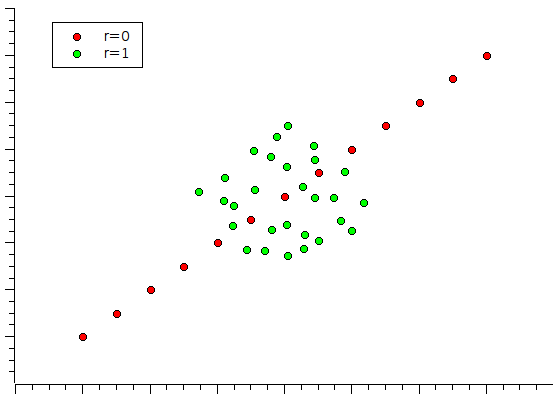
\includegraphics[scale=0.5]{img/correlazione.png}
    \caption{confronto fra correlazione massima e minima\label{fig:confrontomaxminr}}
  \end{figure}
  
Nel caso gaussiano $\hat{X}(y)$ è una funzione lineare di $y$, inoltre, l'errore quadratico medio $E\left[(X-\hat{X}(y))^2|Y=y\right]$ non dipende da $y$: la qualità della stima la conosciamo già prima di avere le osservazioni.\newline
Nel caso più generale (non gaussiano) lo stimatore MS è una funzione non lineare di $y$. Trattando vettori di V.C. congiunte e gaussiani abbiamo:

  \begin{align*}
    Var\begin{bmatrix} X \\ Y\end{bmatrix} &=\begin{bmatrix} V_{XX} & V_{XY} \\ V_{YX} & V_{YY} \end{bmatrix}=\begin{bmatrix} Var[X] & cov[X,Y] \\ cov[Y,X] & var[Y]\end{bmatrix} \\
    E[X|Y=y]&=E[X]+V_{XX} \cdot V_{YY} \cdot (y-E[Y]) \\
    Var\left[(X-\hat{X}|Y=y)\right]&=V_{XX}-V_{XY} \cdot V_{YY}^{-1} \cdot V_YX
  \end{align*}
  
Come abbiamo visto la linearità è solo un caso particolare della gaussianità congiunta, lo stimatore MS è generalmente non lineare e quindi di più difficile trattazione, sia teorica che computazionale. In figura \ref{fig:confrontogaussgenerico} è rappresentato un esempio di angamento gaussiano e un andamento generico.

  \begin{figure}[htbp]
    \centering
    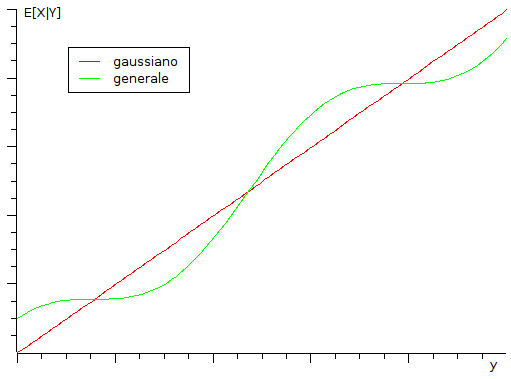
\includegraphics[scale=0.5]{img/gaussgeneral.png}
    \caption{confronto fra il caso gaussiano e quello generico\label{fig:confrontogaussgenerico}}
  \end{figure}

Avere a che fare con problemi lineari è molto più comodo, quindi, anche se il modello ideale è di tipo non lineare vogliamo quindi restringerci alla sola classe degli stimatori lineari - stimatore MS lineare- :

  \[ \hat{X}_L(y)=aY+b \]
  
\paragraph{Teorema} l'errore:

  \[ J=E\left[(X-\hat{X}_L(y))^2\right]=E\left[(X-aY-b)^2\right] \]
  
è minimizzato in corrispondenza di:

  \[ \hat{X}_L(y)=E[X|Y=y]=E[X]+cov(X,Y) \cdot \frac{1}{Var[Y]} \cdot (Y-E[Y])\]
  
Altro non è che la stessa formula del caso gaussiano. Nel caso vettoriale, invece:

  \begin{gather*}
    \hat{X}_L(y)=E[X]+V_{XX} \cdot V_{YY}^{-1} \cdot (Y-E[Y]) \\
    E\left[(X-\hat{X}_L(y))\cdot (X-\hat{X}_L(y))^T\right]=V_{XX}-V_{XY} \cdot V_{YY}^{-1}  \cdot V_{YX}
  \end{gather*}
  
Lo stimatore MS lineare è l'ottimo assoluto nel caso gaussiano, nel caso non gaussiano è ancora ottimo ma limitatamente alla classe degli stimatori lineari.
% ########################################################################
\subsection{Stimatori a posteriori}
Partiamo dal presupposto di aver calcolato, o di conoscere già, la ddp condizionata $f_{\Theta|X}(\theta|X)$ \footnote{ovvero i parametri in funzione dei dati}, come calcoliamo la stima $\hat{\theta}$? Per fare ciò abbiamo diverse alternative
\subsubsection{Stima Maximum A Posteriori - MAP}  %############
\index{Stima maximum a posteriori (MAP)}
  \[ \theta^{MAP}(X)=\arg \max_\theta f_{\Theta|X}(\theta|X) \]
  
Il valore del parametro stimato $\hat{\theta}$ è individuato in corrispondenza della moda della ddp a posteriori.
Per il teorema di Bayes, enunciato precedentemente, il denominatore è un valore indipendente dal parametro $\theta$, quindi non concorre alla determinazione del valore che massimizza la ddp a posteriori:

  \[ f_{\Theta|X}(\theta|X)=\frac{f_{X|\Theta}(X|\theta) \cdot f_\Theta(\theta)}{...} \]
  
quindi possiamo anche scrivere:

  \[ \theta^{MAP}(X)=\arg \max_\theta f_{X|\Theta}(X|\theta) \cdot f_\Theta(\theta) \]
  
Confrontando quest'ultima formulazione della stima MAP notiamo che assomiglia molto alla stima ML, infatti, senza conoscenza a priori sarebbe la formula della verosimiglianza, ma anche nel caso in cui la conoscenza a priori sia uniforme, ovvero $f_\Theta$ è costante.\newline
Come per la stima ML, anche per la stima MAP poterebbe essere più conveniente massimizzare il supporto, inoltre, tutte le tecniche di calcolo numerico adottate per la stima ML sono ancora valide per la stima MAP (di cui la stima ML è un caso particolare).
Come abbiamo visto, la stima MAP usa la moda come parametro di riferimento, ma con alcuni tipi di distribuzione la moda è poco significativa, ad esempio quando la ddp a posteriori è di tipo esponenziale, si avrebbe $\theta^{MAP}=0$ quando, invece, è ben evidente dalla figura \ref{fig:expMAP} che c'è il 100\% di probabilità che ciò non sia vero, ma che $\theta^{MAP}>0$

\begin{center}
\textbf{[FIXME: disegnare la moda sul grafico e scrivere un commento decente]}
\end{center}
\begin{figure}[htbp]
  \centering
  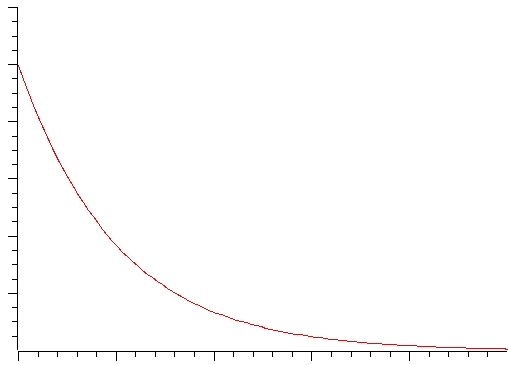
\includegraphics[scale=0.5]{img/exp.png}
  \caption{esponenziale\label{fig:expMAP}}
\end{figure}


\subsubsection{Stima di Bayes - B} %############
\index{Stima di Bayes}
  \[ \theta^B(X)=E[\Theta|X] \]
è lo stimatore in media quadratica. Se $\Theta$ e $X$ sono congiuntamente gaussiane, allora:

  \begin{gather*}
    \theta^B(X)=\theta^{MAP}(X)=E[\Theta]+V_{\Theta X} \cdot V_X^{-1} \cdot (X-E[X])\\
    Var \left[\begin{bmatrix} X \\ \Theta \end{bmatrix} \right]=\begin{bmatrix} V_X \ V_{X\Theta} \\ V_{\Theta X}^T \ V_\Theta \end{bmatrix}
  \end{gather*}
  
Nei casi in cui, invece, non siano congiuntamente gaussiane è raro trovare formulazioni esplicita; questo spiega il successo della stima MAP, infatti, risulta molto più facile risolvere un problema di massimizzazione piuttosto che risolvere l'integrale che richiede la stima di Bayes. Un'altro punto debole della stima di Bayes risiede proprio nell'uso del valore medio, infatti, nei casi in cui la scelta è vincolata a valori discreti la stima di Bayes potrebbe ritornare un valore inesistente, ad esempio: supponendo di avere una moneta e di stimare se è onesta ($\Theta=0$) o truccata ($\Theta=1$) con $p=0.8$, la stima di Bayes risulterebbe $\theta^B=0.2$, che è un risultato senza significato perché noi volevamo una stima sull'onesta: o lo è, o non lo è.
\subsubsection{Stima Mean Square lineare - MS} %############
\index{Stima Mean Square lineare (MS)}
  \[ \theta^{MS}(X)=E[\Theta]+V_{\Theta X} \cdot V_X^{-1} \cdot (X- E[X]) \]
Nel caso in cui $\Theta$ e $X$ siano congiuntamente gaussiani, lo stimatore MS coincide con lo stimatore di Bayes ma anche con lo stimatore MAP, infatti, nel caso gaussiano gli stimatori sono tutti uguali perché media, moda e mediana cadono nello stesso punto.
\subsubsection{Stimatore mediano} %###########

  \[ \hat{\theta}=mediana(f_{\Theta|X}) \]
  
Questo stimatore può avere dei vantaggi rispetto allo stimatore con media perché se vi sono degli outlier molto grandi la media viene influenzata di molto, mentre la mediana no.
% ######################################################################## Conclusioni
\subsection{Conclusioni}
Come conclusione della stima a posteriori cerchiamo di capire quando è utile usarla.

  \begin{itemize}
    \item se il parametro da stimare $\theta$ è una V.C. (ad esempio l'estrazione da una scatola di monete oneste o truccate) 
    \item stima sequenziale, ovvero i dati arrivano dilazionati nel tempo. All'inizio si ha un insieme di dati e si costruisce una prima stima, con l'arrivo di altri dati bisogna ricostruire la stima. Si può procedere in due modi: mettere insieme tutti i dati e rifare la stima; oppure, propagare l'informazione usando la prima stima come stima a priori ed elaborarla assieme ai nuovi dati usandoli come stima a posteriori. 
    \item usiamo $f_{\Theta}$ come conoscenza a priori, questo ha il vantaggio di essere più generale della stima ML e di ottenere risultati anche con pochi dati; di contro si fanno ipotesi molto forti e il problema della scelta della funzione $f_{\Theta}$ 
  \end{itemize}
